%------------------------------------------------------------------------
%Editar Diplomado
\hypertarget{cv:modificarEntidad}{\section{Modificar Entidad}} \label{sec:modificarEntidad}

	Esta funcionalidad le permitirá modificar la información de una entidad previamente registrado con el fin de corregir o actualizar datos del mismo. 

		\subsection{Procedimiento}

			%Pasos de procedimiento
			\begin{enumerate}
	
			\item Oprima el botón \IUEditar{} de algún registro existente de la pantalla \ref{fig:GestionarEntidades} ''Gestionar Entidades''.
	
			\item Se mostrará la pantalla \ref{fig:modificarEntidad} ''Modificar Entidad''.
			
			%Pantalla
			\begin{figure}[htbp!]
				\begin{center}
					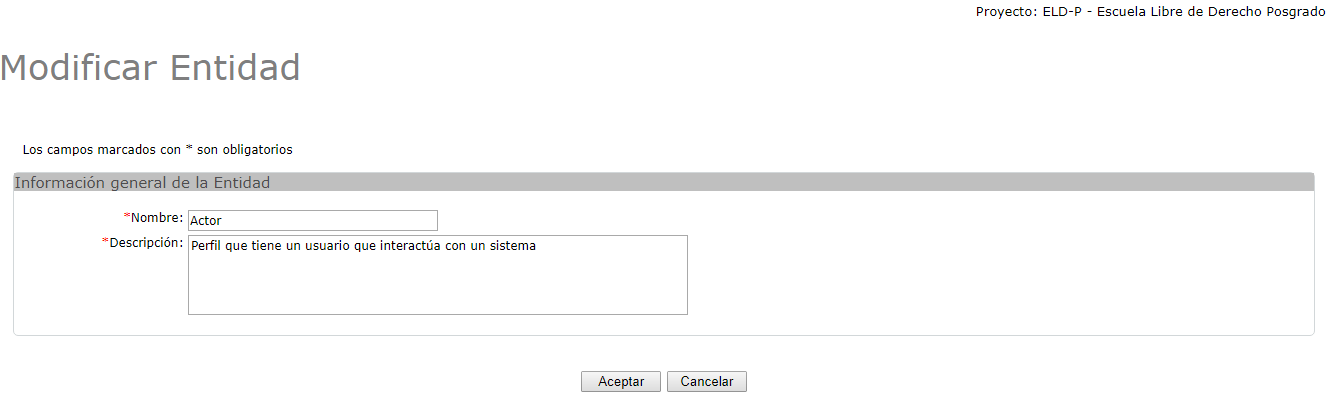
\includegraphics[scale=0.5]{roles/lider/entidades/pantallas/IU12-2modificarEntidad}
					\caption{Modificar Entidad}
					\label{fig:modificarEntidad}
				\end{center}
			\end{figure}
		
			\item Modifique los datos solicitados por la pantalla.
						
			\item Oprima el botón \IUAceptar.
			
			\item Se mostrará el mensaje \ref{fig:entidadModificada} en la pantalla \ref{fig:GestionarEntidades} ''Gestionar Entidades''.
			
			\begin{figure}[htbp!]
				\begin{center}
					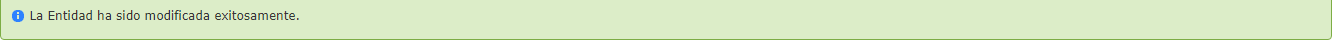
\includegraphics[scale=0.5]{roles/lider/entidades/pantallas/IU12-2MSG1}
					\caption{MSG: Término Actualizado}
					\label{fig:entidadModificada}
				\end{center}
			\end{figure}
			\end{enumerate}